\documentclass{article}
\usepackage{graphicx}
\usepackage{amsmath}
\usepackage[numbers]{natbib}
\usepackage{url}
\usepackage{dirtree}
\usepackage{tikz}
\usepackage{float}
\usepackage{placeins}
\usepackage{xurl}
\usepackage{hyperref}
\clubpenalty=10000
\widowpenalty=10000
\setlength{\emergencystretch}{3em}
\renewcommand{\topfraction}{0.9}
\renewcommand{\bottomfraction}{0.9}
\renewcommand{\textfraction}{0.1}
\renewcommand{\floatpagefraction}{0.8}
\usetikzlibrary{arrows.meta, positioning}

\title{LASPOS:\\A Comprehensive User Guide}
\author{%
  Ha Bao Dao\,$^{1}$, 
  Duc Ninh Le\,$^{2}$
  Huy Hoang Le\,$^{1}$, and
  Minh Bao Nguyen\,$^{1}$\\  [2ex]
  \\
  \small $^{1}$The Dewey Schools Tay Ho: Adventure International Program, Hanoi 11900, Vietnam\\[0.5ex]
  \small $^{2}$Phenikaa Institute for Advanced Study, Phenikaa University, Hanoi 12116, Vietnam
}
\date{}

\begin{document}
\newcommand{\secref}[1]{Section~\ref{#1}}
\maketitle
\newpage
\begin{abstract}
    We present a simplified Monte Carlo simulation of proton--proton collisions at the Large Hadron Collider (LHC), LASPOS (for Large hAdron collider Simplified Particle cOllision Simulator), developed as an educational project at the high-school level under the mentorship of a particle physics researcher. The simulation generates events from a fixed menu of six representative final-state channels, ranging from two to four outgoing particles, at a given center-of-mass energy. Rather than modeling the full matrix-element physics of a real collision, which involves quantum field theory and parton distribution functions far beyond the scope of this project, the simulation enforces only the fundamental conservation laws---energy, momentum, electric charge, baryon number, and lepton number---together with correct relativistic kinematics.

    Multi-particle final states are generated using a sequential two-body decomposition technique: any subset of outgoing particles is treated as a single fictitious composite of randomly drawn invariant mass, reducing an n-body ($n\geq2$) final state to a chain of exactly solvable two-body decays. Each two-body decay is solved in closed form from energy-momentum conservation, and composite systems are decayed in their own rest frame before being transformed back to the laboratory frame via the general $4\times4$ Lorentz boost matrix. This approach guarantees, by construction, that every generated event conserves energy and momentum to numerical precision, and that every outgoing particle is correctly on its mass shell.

    Our program generates a list of events. In the data analysis step, each generated event is subsequently passed through a simplified detector acceptance model, incorporating a set of kinematic cuts, a minimum particle energy threshold and a polar-angle acceptance window that excludes the beam-pipe region, approximating the geometric coverage of a real collider detector such as ATLAS or CMS. Any distribution of the generated events, such as particle energies, angles, transverse momenta, and invariant masses, can then be plotted.

    The accompanying software is organized into three independent stages---event generation, detector-cut filtering, and data visualization---and is accompanied by an automated test suite verifying the physical correctness of the generated events. Beyond its role as a physically accurate illustration of relativistic kinematics, this project is intended to serve as a practical, hands-on introduction to the Monte Carlo event generation and data analysis techniques that underpin experimental particle physics at facilities such as the LHC. Our program is publicly available on GitHub.
    \\\par\smallskip\noindent October 3, 2026
\end{abstract}
\newpage

\tableofcontents
\newpage

\section{Introduction}
\par The Large Hadron Collider (LHC) at CERN is the largest and most powerful particle accelerator in the world \cite{cern_lhc}. Located in a 27-kilometer ring straddling the border between France and Switzerland, it accelerates two counter-rotating beams of protons to extremely high energies and collides them head-on at several interaction points around the ring. By concentrating enormous energy into a vanishingly small volume of space, these collisions allow physicists to probe the fundamental structure of matter at distance scales far smaller than the proton itself, and have enabled the discovery of new fundamental particles that cannot be observed under ordinary conditions. The most celebrated such discovery to date is the Higgs boson, observed independently by the ATLAS and CMS collaborations in 2012 \cite{atlas_higgs, cms_higgs}, which confirmed the mechanism by which elementary particles acquire mass and completed the Standard Model (SM) of particle physics.
\par Understanding what happens inside a single LHC collision, and how a detector reconstructs that collision from the particles it produces, is central to modern experimental particle physics. A proton is not itself a fundamental particle, but a bound state of quarks and gluons; when two protons collide at high energy, it is in reality a single constituent from each proton that interacts, while the remainder of each proton contributes a sub-dominant role. The outcome of such an interaction is fundamentally probabilistic: a wide range of final states, each containing a different combination of particles, is possible, with the frequency of each final state governed by the underlying laws of quantum field theory (QFT). The best simulators using QFT and the SM currently used by particle physicists are Pythia \cite{pythia8}, Herwig \cite{herwig7}, and Sherpa \cite{sherpa3}. They are hugely complicated and need a lot of computer power to run.
\par Reconstructing what occurred, and separating a genuine signal---such as a Higgs boson decaying to two photons---from the far more common background processes that mimic it, is one of the principal challenges of experimental particle physics, and depends critically on the relativistic kinematics of energy, momentum, and mass that any outgoing particle must obey.
\par The full physics governing a real LHC collision, however, involves QFT, parton distribution functions, and detector simulations of enormous complexity, far beyond the scope of a high-school-level project. The purpose of this project is therefore to construct a simplified, self-contained simulation of LHC proton--proton collisions that captures the essential physical principles governing any such collision---conservation of energy, momentum, electric charge, baryon number, and lepton number, together with the relativistic kinematics relating a particle's energy, momentum, and mass, as described by the Lorentz transformation \cite{jackson1998}---while deliberately setting aside the full complexity of the underlying collision dynamics. Rather than attempting to predict which final states occur with physically accurate probabilities, final states are drawn from a fixed, hand-chosen menu, and the resulting kinematics of each event are generated exactly using uniform random number distributions, so that every simulated event is a physically valid outcome even though the relative frequency of different outcomes is illustrative rather than predictive.
\par This simulation is designed first and foremost as an educational tool. Its primary aim is to make the core kinematic principles governing particle collisions---conservation of energy momentum and Lorentz invariance---approachable to a student encountering them for the first time, by grounding each concept directly in a working piece of code that can be run, modified, and inspected. A secondary aim is to serve as a practical introduction to the broader workflow of experimental particle physics: generating a large sample of simulated events, applying a model of detector acceptance to that sample, and extracting physically meaningful distributions from the result, mirroring in miniature the pipeline used by real LHC analyses. Our program LASPOS (for Large hAdron collider Simplified Particle cOllision Simulator) is open source and is available at \url{https://github.com/laspos/laspos}
\par The remainder of this report is organized as follows. \secref{sec:theoretical_background} reviews the atomic, nuclear, and particle-physics background necessary to follow the simulation, including the quark model of hadronic matter. \secref{sec:user_guide} is a practical guide to installing, running, and verifying the accompanying simulation code. \secref{sec:kinematics_framework} develops the relativistic kinematic framework---four-vectors, two-body decay kinematics, and the Lorentz boost---underlying the event generator, with full derivations given in Appendices~\ref{app:2to2}--\ref{app:2to4}. \secref{sec:methods} describes the simulation's methodology in detail: the final-state channels generated, the detector-acceptance model applied, and the event logging procedure. \secref{sec:program_structure} describes the structure of the accompanying software. \secref{sec:numerical_results} presents and discusses the resulting numerical distributions, and \secref{sec:conclusion} summarizes the work and outlines possible extensions.

\section{Theoretical Background}
\label{sec:theoretical_background}

\subsection{Atomic and Nuclear Structure}
\par An atom consists of a positively charged nucleus surrounded by negatively charged N electrons, with a total charge $Q = (+N) + (-N) = 0$ for a neutral atom---the basis of quantum chemistry. The nucleus itself is composed of N protons and a number of neutrons. The simplest case consists of a single proton, while heavier nuclei (e.g., helium) combine multiple protons and neutrons.

\subsection{Hadrons and the Quark Model}
\label{ssec:hadrons&quark}
\par The proton and neutron belong to a broader class of particles called hadrons, which are subdivided into baryons and mesons. Unlike the electron, the proton and neutron are not fundamental---they are composite particles built from quarks and gluons.
\par In the simple (naive) quark model, a proton is composed of two up quarks and one down quark, $p = (uud)$, while a neutron is composed of one up quark and two down quarks, $n = (udd)$. The assignment of the up quark an electric charge of $+2/3$ and the down quark a charge of $-1/3$ \cite{pdg2024} correctly reproduces the observed charges $Q_p = +1$ and $Q_n = 0$. We are using here a unit system where the charge of the electron is -1. This model was developed by Murray Gell-Mann and other scientists \cite{gellmann1964}, a work for which he was awarded the Nobel Prize.
\par A more complete picture accounts for color confinement: quarks carry an additional charge-like quantum number called color, and are bound together by gluons, the massless, electrically neutral carriers of the strong force. In this refined model, the proton is written including a gluon-mediated binding structure between the valence quarks (u,d) rather than as three free particles. And antiquarks carry electric charge opposite in sign but equal in magnitude to their corresponding quarks. Together with valence quarks (e.g., u,d for the proton) there are sea quarks consisting of quark - antiquark pairs. An antiquark is the partner of a quark, which has the same mass but opposite electric charge. A quark - antiquark pair is therefore electrically neutral and does not contribute to the electric charge of a hadron.

\subsection{Conserved Quantities}
\label{ssec:conserved}
In any collision, certain quantities have the same total value before and after the collision. Besides energy and momentum, three of them concern the particles themselves: electric charge, baryon number, and lepton number.

\par\textbf{Electric charge.} The total electric charge $Q$ is the sum of the charges of the particles, in the unit system of \secref{ssec:hadrons&quark} where the charge of the electron is $-1$.

\par\textbf{Baryon number.} The baryon number $B$ counts quarks: each quark carries $B=+1/3$ and each antiquark carries $B=-1/3$. A proton $(uud)$ and a neutron $(udd)$ therefore have $B=+1$, their antiparticles have $B=-1$, and a meson, built from a quark and an antiquark, has $B=0$. Particles that contain no quarks, such as the photon and the leptons, also have $B=0$.

\par\textbf{Lepton number.} The lepton number $L$ counts leptons. Electrons, muons, tau leptons, and their neutrinos carry $L=+1$, their antiparticles (such as the positron and the antimuon) carry $L=-1$, and all other particles, including quarks, photons, and gluons, have $L=0$.

Electric charge is conserved exactly in all known interactions, and no violation of baryon number or lepton number conservation has ever been observed, including in searches for proton decay \cite{pdg2024}. The two incoming protons carry $Q=+2$, $B=+2$, and $L=0$, so every final state must carry the same totals. Because these totals are fixed by the initial state, an extra baryon can only be created together with an antibaryon, and an extra lepton only together with an antilepton. This is why the neutron appears together with an antineutron, and the electron and muon together with their antiparticles, in the final-state menu of \secref{sec:methods}.

\begin{table}[H]
\centering
\begin{tabular}{l c c c}
\hline
Particle & $Q$ & $B$ & $L$ \\
\hline
Proton $p$ & $+1$ & $+1$ & $0$ \\
Neutron $n$ & $0$ & $+1$ & $0$ \\
Antineutron $\overline{n}$ & $0$ & $-1$ & $0$ \\
Electron $e^-$ & $-1$ & $0$ & $+1$ \\
Positron $e^+$ & $+1$ & $0$ & $-1$ \\
Muon $\mu^-$ & $-1$ & $0$ & $+1$ \\
Antimuon $\mu^+$ & $+1$ & $0$ & $-1$ \\
Photon $\gamma$ & $0$ & $0$ & $0$ \\
\hline
\end{tabular}
\caption{Electric charge $Q$, baryon number $B$, and lepton number $L$ of the particles that appear in the simulation.}
\label{tab:quantum_numbers}
\end{table}

Adding up the entries of Table~\ref{tab:quantum_numbers} shows that every final state in the menu has $Q=+2$, $B=+2$, and $L=0$. For example, $pp\,e^+e^-$ has $Q=1+1+1-1=+2$, $B=1+1=+2$, and $L=-1+1=0$, whereas a final state $ppnn$ would have $B=+4$ and is forbidden. In the simulation, energy and momentum conservation is enforced by the kinematic procedure of \secref{sec:kinematics_framework}, while conservation of charge, baryon number, and lepton number follows from the choice of final states.

\section{Running the Simulation: A User Guide}
\label{sec:user_guide}

This section explains how to obtain, configure, and run the simulation code accompanying this report, and how to reproduce the figures discussed in later sections. The code is organized into three independent stages---event generation, detector-cut filtering, and plotting---each of which reads a file written by the previous stage and writes a file for the next, so that any stage can be re-run on its own without repeating the others.

\subsection{Obtaining the Code and Installing Requirements}
\label{ssec:requirements}
The complete source code is available on GitHub at \url{https://github.com/laspos/laspos}. It can be downloaded as a ZIP archive from the repository page (\textit{Code}, then \textit{Download ZIP}), or cloned with Git using the command \texttt{git clone} followed by the repository address.

The simulation requires Python 3.8 or newer. The event generator itself uses only the Python standard library; the analysis and plotting scripts additionally require \texttt{numpy} (version 1.24 or newer) and \texttt{matplotlib} (version 3.7 or newer). From inside the project folder, a virtual environment should be created and the two packages installed:
\begin{verbatim}
python -m venv .venv
.venv\Scripts\Activate.ps1      # Windows PowerShell
source .venv/bin/activate       # macOS / Linux
pip install "numpy>=1.24" "matplotlib>=3.7"
\end{verbatim}
No data needs to be regenerated to begin exploring the project: a dataset of 100{,}000 collision events, together with the figures derived from it, is included with the code.

\subsection{Project Organization}
\label{ssec:organization}
The code is divided into three stages, each corresponding to one physical step of the analysis: generating collisions, filtering them through a simplified detector model, and producing histograms from the result.
\begin{itemize}
    \item \texttt{simulation.py} (Stage 1) generates collision events according to the final-state menu and kinematic procedures of \secref{sec:kinematics_framework} and \secref{sec:methods}, and writes them, unfiltered, to \texttt{collision\_data/events.txt}.
    \item \texttt{analysis.py} (Stage 2) reads a plain-text settings file, \texttt{analysis\_card.txt}, applies the detector acceptance cuts described in \secref{ssec:detector_model}, and writes the surviving events to \url{analysis_tools/analysis_data/events_analysed.txt}.
    \item The scripts in \texttt{analysis\_tools/} (Stage 3) read an events file and produce histograms of particle energies, angles, transverse momenta, and invariant masses, saved as image files under \texttt{plots/}.
\end{itemize}
The physics itself---four-momenta, two-body decays, Lorentz boosts, and invariant mass---is implemented separately in \texttt{utilities/kinematics.py}, which deals only in numerical quantities and has no knowledge of particle names; \texttt{simulation.py} is responsible for choosing which particles appear and recording the result.

\subsection{Stage 1: Generating Collision Events}
\label{ssec:running_stage1}
Running
\begin{verbatim}
python simulation.py
\end{verbatim}
repeatedly generates collisions until a target number of events, set by \texttt{TARGET\_LOGGED\_EVENTS} near the top of the file, have been written. No detector cuts are applied at this stage: the only event ever discarded is one that fails an internal energy-and-momentum conservation check, which would indicate a bug rather than a physical limitation. Three settings may be adjusted directly in \texttt{simulation.py}:
\begin{itemize}
    \item \texttt{TARGET\_LOGGED\_EVENTS}---the number of events to generate. A larger number produces smoother histograms at the cost of longer runtime and a larger output file.
    \item \texttt{TOTAL\_ENERGY}---the collision energy in TeV, set by default to 13.6 TeV, the LHC's current operating energy.
    \item \texttt{SEED}---a fixed random seed, so that the same value reproduces an identical dataset; setting it to \texttt{None} produces a fresh, non-reproducible sample each run.
\end{itemize}
Re-running this script overwrites the existing \texttt{events.txt}, so the file should be copied first if a prior dataset is to be preserved for comparison.

\subsection{Stage 2: Applying Detector Acceptance Cuts}
\label{ssec:running_stage2}
The acceptance cuts described in \secref{ssec:detector_model} are not applied during event generation; they are applied afterward, by
\begin{verbatim}
python analysis.py
\end{verbatim}
which reads its settings from \texttt{analysis\_card.txt}, a plain-text file with one setting per line. The available cuts are a minimum particle energy, a polar-angle acceptance window, a pseudorapidity limit, and a minimum transverse momentum; each may be independently enabled or disabled, and an event is kept only if every one of its particles passes every enabled cut. Editing the card and re-running \texttt{analysis.py} is sufficient to test a different set of cuts---the underlying collisions do not need to be regenerated. The script reports, per final-state channel, how many events and how many individual particles survived, and writes the surviving events to \url{analysis_tools/analysis_data/events_analysed.txt} in the same format as the input file. The same card can also restrict the analysis to chosen collision types: the \texttt{final\_state} setting takes the identifiers of Table~\ref{tab:channels} (one identifier, several separated by commas, or \texttt{all}), and the script reports how many events of each chosen type were in the file and how many pass the cuts.

\subsection{Stage 3: Producing the Plots}
\label{ssec:running_stage3}
Four scripts under \texttt{analysis\_tools/} produce the figures discussed in \secref{sec:numerical_results}:
\begin{verbatim}
python analysis_tools/graph_energy_steps.py
python analysis_tools/graph_angle_steps.py
python analysis_tools/graph_pt_steps.py
python analysis_tools/graph_mass_steps.py
\end{verbatim}
Each script reads an events file, groups particles by final-state channel and position, and writes one set of figures per process into its own subfolder of \texttt{plots/}. By default, all four scripts read the unfiltered \texttt{events.txt}; changing a single path near the top of each script to point to \texttt{events\_analysed.txt} instead produces the corresponding figures for the cut dataset. The four scripts are independent of one another and may be run in any order.

\subsection{Verifying the Installation}
\label{ssec:running_tests}
An automated test suite is provided under \texttt{tests/}, checking that energy and momentum are conserved in every generated event, that particle directions are correctly isotropic, that the detector cuts are applied correctly, and that the output files are read back consistently. The full suite is run with
\begin{verbatim}
python -m unittest
\end{verbatim}
and is expected to complete in a few seconds with no failures. Running it after any modification to the generation or analysis code is a useful way to confirm that the change has not broken an existing physical or logical guarantee.

\subsection{A First Check of the Output}
\label{ssec:first_check}
Before examining the physics results in \secref{sec:numerical_results}, two quick checks confirm that a dataset was generated and read correctly. First, every event's particle energies should sum to the total collision energy, and its momentum components should each sum to zero; this is checked automatically during generation (\secref{ssec:running_stage1}) but can also be verified by hand on any single event in the output file. Second, the distribution of $\cos\theta$ over many events should be flat: because particle directions are generated with no preferred orientation, a flat $\cos\theta$ histogram is the direct signature of correctly isotropic sampling, while the polar angle $\theta$ itself is expected to peak near $90^\circ$ for purely geometric reasons (a sphere has more surface area near its equator than near its poles). A $\theta$ histogram that comes out flat, or a $\cos\theta$ histogram that does not, indicates a problem with event generation rather than with the physics being modeled.

\section{Mathematical and Physical Foundation}
\label{sec:kinematics_framework}

\subsection{Four-momentum and Invariant Mass}
In general, an energy-momentum four-vector has three independent spatial components:
\begin{equation}
    P = P_\mu = (E,\, p_x,\, p_y,\, p_z),
\end{equation}
where $\vec{p} = (p_x, p_y, p_z)$ is the full spatial three-vector. We take the flight direction of incoming proton 1 to define the $+z$ axis (with proton 2 travelling in the $-z$ direction), consistent with the beam-axis convention used throughout this report.

\paragraph{Spherical coordinates.} For an outgoing particle with four-vector $q_\mu = q = (E_q, q_x, q_y, q_z)$, it is often convenient to describe the spatial vector $\vec{q}$ using spherical coordinates $(|\vec{q}|, \theta, \varphi)$ instead of Cartesian coordinates $(q_x, q_y, q_z)$, where
\begin{equation}
    |\vec{q}| = \sqrt{q_x^2 + q_y^2 + q_z^2}
\end{equation}
is the magnitude of $\vec{q}$, $\theta = \angle(\vec{q}, Oz)$ is the polar angle measured from the beam axis, and $\varphi = \angle(Ox, \vec{q}\,')$ is the azimuthal angle measured from the $x$-axis to the projection $\vec{q}\,'$ of $\vec{q}$ onto the transverse $(x,y)$ plane. These range over
\begin{equation}
    |\vec{q}| \geq 0, \qquad \theta \in [0, \pi], \qquad \varphi \in [0, 2\pi) \;\; (\text{or equivalently } (-\pi, \pi]).
\end{equation}
The Cartesian and spherical descriptions are related by
\begin{equation}
    q_z = |\vec{q}|\cos\theta, \qquad q_x = |\vec{q}|\sin\theta\cos\varphi, \qquad q_y = |\vec{q}|\sin\theta\sin\varphi.
\end{equation}
\par\textbf{Isotropic directions.}\label{para:isotropic}
Whenever this report says that a direction is drawn randomly, it is drawn isotropically, meaning that no direction is preferred and the probability of a direction is proportional to the solid angle it covers,
\begin{equation}
    dP = \frac{d\Omega}{4\pi} = \frac{\sin\theta\,d\theta\,d\varphi}{4\pi}.
\end{equation}
Equivalently, $\cos\theta$ is uniformly distributed in $[-1,1]$ and $\varphi$ is uniformly distributed in $[0,2\pi)$. The ranges $\theta\in[0,\pi]$ and $\varphi\in[0,2\pi)$ quoted in the following sections are the allowed values of the angles, not a statement that $\theta$ itself is uniform. Because of the factor $\sin\theta$, the distribution of $\theta$ peaks at $90^\circ$, while the distribution of $\cos\theta$ is flat (\secref{ssec:first_check}).

\paragraph{Scalar product and invariant mass.} The Minkowski scalar product of two four-vectors $P_\mu = (E_p, p_x, p_y, p_z)$ and $q_\mu = (E_q, q_x, q_y, q_z)$ is
\begin{equation}
    P_\mu \cdot q_\mu = E_p E_q - p_x q_x - p_y q_y - p_z q_z,
\end{equation}
so that the invariant mass of a two-particle system $(p,q)$ is
\begin{equation}
    m_{pq} = \sqrt{(p+q)^2} = \sqrt{(E_p+E_q)^2 - (p_x+q_x)^2 - (p_y+q_y)^2 - (p_z+q_z)^2}.
\end{equation}
For a massless particle of momentum $P$, this reduces to
\begin{equation}
    m^2 = P^2 = E_p^2 - p_x^2 - p_y^2 - p_z^2 = 0 \quad \Rightarrow \quad |\vec{p}| = E_p,
\end{equation}
consistent with the massless result of \secref{sssec:2to2}.

\subsection{Two-Body Kinematics (2-to-2)}
\label{sssec:2to2}
Consider a collision $p_1 + p_2 \rightarrow B + C$ in the center-of-mass frame, where the incoming four-momenta are $P_{1\mu}=(E,0,0,E)$
 and $P_{2\mu}=(E,0,0,-E)$, so that the total energy is $2E$ and the total momentum vanishes $\vec{p}_1 + \vec{p}_2 = 0$.
\par\textbf{Massless case.} If both outgoing particles are massless ($P_B^2 = P_C^2 =0$), momentum conservation $\vec{p}_B + \vec{p}_C=0$ combined with $E_B=|\vec{p}_B|$, $E_C = |\vec{p}_C|$ forces
 \begin{equation}
     E_B = E_C = E,
 \end{equation}
with the emission direction of $B$ drawn isotropically (\secref{para:isotropic}), and $C$ emitted back-to-back ($\theta_C = \pi - \theta_B$, $\varphi_C = \varphi_B + \pi$).
\par\textbf{Massive case.} If B and C carry masses $m_B \neq m_C$, the on-shell conditions $E_B^2 - |\vec{p}|^2 = m_B^2$ and $E_C^2 - |\vec{p}|^2 = m_C^2$ (with $|\vec{p}_B| = |\vec{p}_C| = |\vec{p}|$, since the two momenta are equal and opposite) combine with energy conservation $E_B+E_C=2E$ to give
\begin{equation}
\begin{gathered}
    E_B = \frac{1}{2}[2E + \frac{m_B^2 - m_C^2}{2E}],\\
    E_C = \frac{1}{2}[2E - \frac{m_B^2 - m_C^2}{2E}].
\end{gathered}
\end{equation}
In general $E_B \neq E_C$ when $m_B \neq m_C$; the massless result above is recovered as the special case $m_B = m_C$ (in particular $m_B = m_C = 0$). The full step-by-step derivation of these results is given in Appendix~\ref{app:2to2}.


\subsection{Multi-Body Final States via Sequential Two-Body Decomposition}
For final states with more than two particles, we exploit the fact that any subset of outgoing particles can be treated as a single fictitious composite particle carrying a variable invariant mass, reducing the problem to a chain of ordinary 2-to-2 decays \cite{byckling_kajantie}.
\par\textbf{Three-body final states (2-to-3).}
\label{para:2to3} For $p_1 + p_2 \rightarrow 3+4+5$, particle 3 is treated as one outgoing body and particles 4 and 5 are grouped into a composite "particle" of invariant mass $m_{45} \in [0,2E]$. The reaction is then treated as an effective two-body process $p_1 + p_2 \rightarrow 3+(45)$:
\begin{enumerate}
    \item Apply the two-body formulas of \secref{sssec:2to2} with $B=3$ (massless, $m_3 = 0$) and $C=(45)$ (mass $m_{45}$) to obtain $E_3$ and $E_{45}$, with emission direction $(\theta_3, \varphi_3)$ drawn from $\theta_3 \in [0,\pi]$, $\varphi_3 \in [0, 2\pi)$, and $(45)$ emitted back-to-back, $\theta_{45} = \pi - \theta_3$, $\varphi_{45} = \varphi_3 + \pi$.
    \item In the rest frame of the (45) system, particles 4 and 5 are emitted back-to-back with $E'_4 = E'_5 = m_{45}/2$ and a random direction $(\theta'_4, \varphi'_4)$, following the massless two-body case of \secref{sssec:2to2} (with $m_{45}$ playing the role of the total energy budget in that frame).
    \item The four-momentum $P'_4$ is boosted from the (45)-rest frame back to the lab frame $R_{12}$ using the boost matrix defined in \secref{sssec:lorentz}, with the boost velocity fixed by $P_{45}$ as measured in the lab frame (lab frame = $R_{12}$ frame = center of mass frame of $(1,2)$). $P_5$ is then obtained either by an identical boost of $P'_5$, or directly from momentum conservation $P_5=P_{45}-P_4$. The full step-by-step derivation of this procedure is given in Appendix \ref{app:2to3}.
\end{enumerate}
\par\textbf{Four-body final states (2-to-4).}
\label{para:2to4} The same strategy extends to $p_1 + p_2 \rightarrow 3+4+5+6$ by grouping the final state into two composite pairs, (34) and (56):
\begin{enumerate}
    \item Draw $m_{34} \in [0,2E]$ and $m_{56} \in [0,2E-m_{34}]$, and apply the massive two-body formulas of \secref{sssec:2to2} to the effective process  $p_1 + p_2 \rightarrow (34)+(56)$, obtaining $E_{34},E_{56}$, and a random splitting direction $(\theta_{34}, \varphi_{34}) \in [0,\pi]\times[0,2\pi)$ (with $(56)$ emitted back-to-back, $\theta_{56} = \pi - \theta_{34}$, $\varphi_{56} = \varphi_{34} + \pi$).
    \item Independently decay each composite in its own rest frame, $(34) \rightarrow 3+4$ and $(56) \rightarrow 5+6$, using the two-body relations of \secref{sssec:2to2} (each with its own random direction), yielding primed four-momenta in each composite's rest frame.
    \item Boost each daughter four-momentum back to the lab frame using a boost matrix constructed from the lab-frame momentum of its respective parent composite ($A_{34}$ for (34), $A_{56}$ for (56)), as detailed in \secref{sssec:lorentz}. The full step-by-step derivation of this procedure is given in Appendix \ref{app:2to4}.
\end{enumerate}
This recursive two-body decomposition generalizes to any final-state multiplicity by repeated pairing and boosting.

\subsection{The Lorentz Boost Matrix}
\label{sssec:lorentz}
To transform a four-momentum from the rest frame of a composite system A back to the lab frame $R_{12}$, we use the fact that if $P_A=(E_A,P_{Ax},P_{Ay},P_{Az})$ is the composite's known four-momentum in the lab frame, then any daughter four-momentum $q'$ known in A's rest frame transforms as
\begin{equation}
    q=[A]q', \label{equa:matrixq}
\end{equation}
where $[A]$ is the $4\times4$ boost matrix determined entirely by $P_A$. Defining the boost velocity components
\begin{equation}
\begin{gathered}
    \beta_x=\frac{P_{Ax}}{E_A}, \qquad \beta_y=\frac{P_{Ay}}{E_A}, \qquad \beta_z=\frac{P_{Az}}{E_A}, \\ X=\beta^2_x+\beta^2_y+\beta^2_z, \qquad \gamma=\frac{1}{\sqrt{1-X}},
\end{gathered}
\end{equation}
the matrix elements are
\begin{equation}
\begin{gathered}
    a_{11}=\gamma, \quad a_{12}=\gamma\beta_x, \quad a_{13}=\gamma\beta_y, \quad a_{14}=\gamma\beta_z,\\
    a_{21}=\gamma\beta_x, \quad a_{22}=1+\beta^2_x\frac{\gamma-1}{X}, \quad a_{23}=\beta_x\beta_y\frac{\gamma-1}{X}, \quad a_{24}=\beta_x\beta_z\frac{\gamma-1}{X}, \\
    a_{31}=\gamma\beta_y, \quad a_{32}=\beta_y\beta_x\frac{\gamma-1}{X}, \quad a_{33}=1+\beta^2_y\frac{\gamma-1}{X}, \quad a_{34}=\beta_y\beta_z\frac{\gamma-1}{X}, \\
    a_{41}=\gamma\beta_z, \quad a_{42}=\beta_z\beta_x\frac{\gamma-1}{X}, \quad a_{43}=\beta_z\beta_y\frac{\gamma-1}{X}, \quad a_{44}=1+\beta^2_z\frac{\gamma-1}{X}.
\end{gathered}
\end{equation}
This is the general form of a Lorentz boost along an arbitrary direction set by $(\beta_x,\beta_y,\beta_z)$, which is necessary here since the composite systems' momenta are not in general aligned with the beam axis.

\section{Methods}
\label{sec:methods}

\subsection{Event Generation}
\label{ssec:event_generation}
\par We developed a Monte Carlo simulator in Python to generate proton--proton collision events at any center-of-mass energy (default choice is the current LHC evergy of $\sqrt{s} = 13.6$~TeV). For each simulated collision, a final-state topology is drawn from a discrete set of six channels, each assigned a fixed sampling probability (Table~\ref{tab:channels}).

\begin{table}[H]
\centering
\begin{tabular}{l|c|c|c|c|c|c}
\hline
\textbf{Process} & $pp$ & $pp\gamma$ & $ppn\overline{n}$ & $ppe^+e^-$ & $pp\mu^+\mu^-$ & $pp\gamma\gamma$\\
\hline
\textbf{ID} & 1 & 2 & 3 & 4 & 5 & 6\\
\textbf{Probability} & 0.25 & 0.22 & 0.18 & 0.15 & 0.15 & 0.05\\
\hline
\end{tabular}
\caption{The six final-state channels, their IDs, and their sampling probabilities. The probabilities are fixed in \texttt{simulation.py}; the ID is used to select a channel in the data analysis step (\secref{ssec:running_stage2}).}
\label{tab:channels}
\end{table}

\par The channel is chosen with a single random number $r$ drawn uniformly from $[0, 1)$. The unit interval is divided into six consecutive sub-intervals whose lengths equal the six probabilities, and the event is assigned the channel whose sub-interval contains $r$. On average, therefore, one collision in four produces the $pp$ final state, and one in twenty produces $pp\gamma\gamma$. The channel fractions actually obtained in our dataset are compared with these probabilities in \secref{ssec:dataset}.

\par All six final states contain two outgoing protons, together with zero to two additional particles. The menu is chosen so that every channel conserves electric charge, baryon number, and lepton number (see \secref{ssec:conserved}), while energy and momentum conservation is enforced exactly by the kinematic procedure of \secref{sec:kinematics_framework}.

\par The $pp$ channel is the only true two-body final state among the six, and is generated directly via the two-body formulas of \secref{sssec:2to2}: each proton receives exactly half of the collision energy, $E = 6.8$~TeV, and the two fly apart back to back along a direction drawn isotropically, with $\cos\theta$ uniform in $[-1, 1]$ and $\varphi$ uniform in $[0, 2\pi)$. The three- and four-particle channels are generated via the sequential two-body decomposition of \secref{para:2to3}, using the Lorentz boost of \secref{sssec:lorentz}; the full derivations are given in Appendices~\ref{app:2to2}--\ref{app:2to4}.

\par In the three-particle channel ($pp\gamma$), particles 4 and 5 are first combined into a composite system of invariant mass $m_{45}$, drawn uniformly between $1$~GeV and $13.6$~TeV. The collision is split into particle 3 and this composite, and the composite is then decayed isotropically in its own rest frame and boosted back into the laboratory frame. In the four-particle channels, particles 3 and 4 form one composite and particles 5 and 6 another. Their masses are drawn one after the other: first $m_{34}$, uniformly between $1$~GeV and $\sqrt{s} - 1$~GeV, and then $m_{56}$, uniformly between $1$~GeV and $\sqrt{s} - m_{34}$. This guarantees $m_{34} + m_{56} \le \sqrt{s}$, so that the split of the collision into the two composites is kinematically allowed. The lower limit of $1$~GeV prevents a composite of exactly zero mass, for which the Lorentz boost would be singular.

\par Drawing the two composite masses in sequence is a simplification, and it makes the four-particle channels asymmetric. The first mass is drawn from the full range, so its mean is $\sqrt{s}/2 = 6.8$~TeV, whereas the second is drawn from whatever range remains, so its mean is only $\sqrt{s}/4 = 3.4$~TeV. Particles 3 and 4 therefore carry more energy on average than the two protons, particles 5 and 6, even though the two pairs play equivalent roles. The size of this effect in the generated data is shown in \secref{ssec:dataset}. A symmetric treatment would draw both masses jointly from the allowed region $m_{34} + m_{56} \le \sqrt{s}$.

\par All outgoing particles are treated as massless, so that $E = |\vec{p}|$; only the intermediate composite systems of \secref{para:2to3} carry an invariant mass. The heaviest outgoing particles, the proton and the neutron, have masses of about $0.94$~GeV, which is negligible next to the TeV-scale energies of most particles: for a proton carrying $6.8$~TeV, $m_p/E \approx 1.4 \times 10^{-4}$. The approximation breaks down only for the softest particles, which can be generated with less energy than their real rest mass. Such particles are removed by the default transverse-momentum cut (\secref{ssec:detector_model}): since $p_T \le E$, every particle that passes $p_T \ge 0.1$~TeV has $E \ge 0.1$~TeV, so $m_p/E \le 0.0094$ for every accepted particle.

\par The random number generator can be given a fixed seed (\texttt{SEED} in \texttt{simulation.py}, default 2026). A run made with a fixed seed is exactly reproducible: running the program again produces the same events.

\subsection{Detector Acceptance Model}
\label{ssec:detector_model}
Real detectors cannot see every particle that a collision produces, so the simulation includes a simplified model of detector acceptance. In the program this model is kept deliberately separate from event generation: the generator writes every collision it makes, unfiltered, and the cuts are applied afterwards, in the data analysis step (\secref{ssec:running_stage2}). Generating events is the slow part of the workflow, so this separation allows many different sets of cuts to be tested on the same dataset without regenerating any collisions. It also mirrors a real experiment, where the detector records everything it can and the choice of cuts is made later by the analyst.

Four cuts are available (Table~\ref{tab:cuts}). Each can be switched on or off independently in the settings file \texttt{analysis\_card.txt}, and a particle is accepted only if it satisfies every cut that is switched on. The analysis step can additionally restrict the output to chosen collision types, selected by the IDs of Table~\ref{tab:channels}.

\begin{table}[H]
\centering
\begin{tabular}{l c c}
\hline
Cut & Condition for acceptance & Default \\
\hline
Pseudorapidity & $|\eta| < \eta_{\max}$ & $\eta_{\max} = 2.5$ \\
Transverse momentum & $p_T \ge p_T^{\min}$ & $0.1$ TeV \\
Minimum energy & $E \ge E_{\min}$ & off \\
Polar-angle window & $\theta_{\min} \le \theta \le \theta_{\max}$ & off ($0^\circ$ to $180^\circ$) \\
\hline
\end{tabular}
\caption{Detector cuts available in the data analysis step, the condition a particle must satisfy to pass each one, and their default settings.}
\label{tab:cuts}
\end{table}

\par\textbf{Pseudorapidity.} The pseudorapidity is the polar angle $\theta$ (measured from the beam axis, see \secref{sec:kinematics_framework}) rewritten in the variable conventionally used at hadron colliders,
\begin{equation}
    \eta = -\ln\!\left[\tan\frac{\theta}{2}\right],
\end{equation}
so that $\theta = 90^\circ$ corresponds to $\eta = 0$, and particles close to the beam axis have large $|\eta|$. The default limit $|\eta| < 2.5$ is the standard coverage of the inner detectors of ATLAS and CMS, and is equivalent to the polar-angle window $9.385^\circ < \theta < 170.615^\circ$. It therefore acts as a beam-pipe cut: particles closer to the beam line than about $9^\circ$ escape down the beam pipe and are not detected. In the program, $\eta$ is computed in the equivalent form $\eta = \frac{1}{2}\ln\left[(|\vec{p}| + p_z)/(|\vec{p}| - p_z)\right]$, which remains numerically accurate for particles very close to the beam axis.

\par\textbf{Transverse momentum.} The transverse momentum is the part of the momentum perpendicular to the beam,
\begin{equation}
    p_T = \sqrt{p_x^2 + p_y^2} = |\vec{p}|\sin\theta = E\sin\theta,
\end{equation}
where the last equality uses $|\vec{p}| = E$ for the massless outgoing particles of this simulation. Transverse momentum is the natural variable at a hadron collider. In a real collision, the colliding partons carry unknown fractions of the proton momenta along the beam, so the total longitudinal momentum of the final state is not known, whereas the total transverse momentum is zero before the collision and must remain so afterwards. Particles with small $p_T$ also travel close to the beam line, where they are hard to reconstruct, and real experiments select particles by their $p_T$. Because $p_T = E\sin\theta$, a cut on $p_T$ acts as an energy cut that tightens towards the beam: with $p_T^{\min} = 0.1$~TeV, a particle at $\theta = 90^\circ$ needs only $0.1$~TeV, whereas a particle at $\theta = 30^\circ$ must carry at least $0.2$~TeV.

\par\textbf{Minimum energy and polar-angle window.} The remaining two cuts are simpler. The minimum-energy cut discards any particle with $E < E_{\min}$, modeling very soft particles lost in detector noise; unlike the $p_T$ cut, it ignores direction entirely. The polar-angle window is the beam-pipe cut written directly in degrees rather than in pseudorapidity, so it is normally used instead of the pseudorapidity cut, not together with it.

None of the cuts depends on the azimuthal angle $\varphi$. This is deliberate: the beam pipe is a hole along the beam axis, which removes a cone at small $\theta$ rather than a wedge in $\varphi$, and a real detector is built symmetrically around the beam. The default configuration applies the pseudorapidity cut $|\eta| < 2.5$ and the transverse-momentum cut $p_T \ge 0.1$~TeV, with the other two cuts switched off, and keeps all six collision types.

\par\textbf{When a particle is accepted and when it is cut.} For every event, the data analysis step applies the following rules, in order.
\begin{enumerate}
    \item If particular collision types have been chosen (the setting \texttt{final\_state} in \texttt{analysis\_card.txt}), an event of any other type is discarded immediately, without its particles being examined.
    \item Each outgoing particle is tested against every cut that is switched on. It is rejected if $E < E_{\min}$, if $\theta$ lies outside the window from $\theta_{\min}$ to $\theta_{\max}$, if $p_T < p_T^{\min}$, or if $|\eta| \ge \eta_{\max}$; otherwise it is accepted. A particle lying exactly on a boundary is therefore accepted, except at $|\eta| = \eta_{\max}$.
    \item The event is kept only if every one of its outgoing particles is accepted. If even one particle is rejected, the whole event is discarded.
\end{enumerate}
A cut is switched off by giving it a value it can never fail: $E_{\min} = 0$, $p_T^{\min} = 0$, a window from $0^\circ$ to $180^\circ$, or \texttt{none} for $\eta_{\max}$. An invalid value, or a misspelled setting name, stops the program with an error rather than being silently ignored, so a cut can never fail to apply without the user noticing.

\subsection{Event Logging and Output Files}
\label{ssec:event_logging}
The generator (\texttt{simulation.py}) applies no detector cuts. For every simulated collision it checks that the total energy equals $13.6$~TeV and that each component of the total momentum vanishes, both to within an absolute tolerance of $10^{-6}$~TeV, and then writes the event to \texttt{collision\_data/events.txt}. The only events discarded are those that fail this check, which would indicate a numerical or programming error rather than a physical effect; in practice no event fails it, and the number of collisions attempted equals the number written. The run continues until a target number of events, 100{,}000 by default (\texttt{TARGET\_LOGGED\_EVENTS} in \texttt{simulation.py}), has been logged.

Each event is stored as a block containing an event identifier, the number of particles, a column header, and one row per outgoing particle giving its name, its energy (TeV), its polar and azimuthal angles (degrees), and its momentum components $p_x$, $p_y$, $p_z$ (TeV), written with six decimal places. For example, the first event of our dataset, a $pp$ event, reads:

{\fontsize{8}{8.5}\selectfont
\begin{verbatim}
___EVENT_ID: 1___
N_Particles: 2
Particle   Energy(TeV)  Theta(deg)   Phi(deg)     p_x(TeV)   p_y(TeV)   p_z(TeV)
proton     6.800000     107.822023   120.218330   -3.258180  5.593997   -2.081216
proton     6.800000     72.177977    300.218330   3.258180   -5.593997  2.081216
\end{verbatim}
}

\noindent The two protons each carry exactly half of the collision energy and fly apart back to back: their polar angles add up to $180^\circ$, their azimuthal angles differ by $180^\circ$, and their momentum components are equal and opposite.

Six decimal places correspond to a precision of $10^{-6}$~TeV, or $1$~MeV, on each stored quantity. This is ample for energies and momenta, but the rounding is amplified when an invariant mass is computed as $m = \sqrt{E^2 - |\vec{p}|^2}$ from TeV-scale values, and it sets a floor of a few GeV on the resolution of any invariant mass reconstructed from the file. This floor is quantified in \secref{ssec:dataset}; it is negligible for the TeV-scale composite masses studied here.

\par\textbf{Where the results are stored.} Each stage of the program writes its results to a fixed location, summarized in Table~\ref{tab:modules}. Every output is overwritten when its stage is run again. The event file written by the analysis step has exactly the same format as \texttt{events.txt}, so the plotting scripts can read either one; in it, the surviving events are grouped by their number of particles and renumbered from 1. In addition, the analysis step prints a summary to the terminal, giving for each channel the number of events kept and the fraction of events and particles that pass.

\begin{table}[H]
\centering
\footnotesize
\begin{tabular}{p{0.25\linewidth} p{0.22\linewidth} p{0.21\linewidth} p{0.22\linewidth}}
\hline
File & Role & Reads & Writes \\
\hline
\texttt{simulation.py} & Stage 1: generate collisions, no cuts & --- & \texttt{collision\_data/\allowbreak events.txt} \\
\texttt{analysis.py} & Stage 2: choose collision types, apply cuts & \texttt{events.txt}, \texttt{analysis\_card.txt} & \texttt{analysis\_tools/\allowbreak analysis\_data/\allowbreak events\_analysed.txt} \\
\texttt{graph\_*\_steps.py} (four scripts) & Stage 3: draw figures & \texttt{events.txt} or \texttt{events\_analysed.txt} & \texttt{plots/}, one folder per process \\
\texttt{kinematics.py} & Physics engine, all stages & --- & --- \\
\texttt{event\_data.py}, \texttt{step\_plot.py} & Reader and plotting library & any events file & --- \\
\hline
\end{tabular}
\caption{The role of each Python file, and the files it reads and writes.}
\label{tab:modules}
\end{table}

\section{The Program Structure}
\label{sec:program_structure}

\subsection{Code Structure}
\label{ssec:code_structure}
The project is organized around the three stages described in \secref{sec:user_guide}. The entry points of Stages~1 and~2, \texttt{simulation.py} and \texttt{analysis.py}, sit at the top level of the project, while the four plotting scripts of Stage~3 sit in \texttt{analysis\_tools/}, together with the code they share. The stages communicate only through files: no stage calls another stage's script, so any stage can be re-run on its own. The only code they share is the physics engine, \texttt{utilities/\allowbreak kinematics.py}, and the file reader, \texttt{analysis\_tools/\allowbreak event\_data.py}. The complete layout is shown in Figure~\ref{fig:dirtree}, and the role of each file is summarized in Table~\ref{tab:modules}.

\begin{figure}[H]
\centering
\begin{minipage}{0.95\textwidth}
\footnotesize
\dirtree{%
.1 {LHC Simulation/}.
.2 {simulation.py \DTcomment{Stage 1: generate events, no cuts}}.
.2 {analysis.py \DTcomment{Stage 2: apply the cuts}}.
.2 {analysis\_card.txt \DTcomment{collision types and cut settings (edit this file)}}.
.2 {README.md \DTcomment{quick start and full documentation}}.
.2 {utilities/}.
.3 {kinematics.py \DTcomment{the physics engine}}.
.2 {analysis\_tools/ \DTcomment{Stage 3: plotting code, and the cut events}}.
.3 {analysis\_data/}.
.4 {events\_analysed.txt \DTcomment{events passing the cuts}}.
.3 {event\_data.py \DTcomment{reads an events file}}.
.3 {step\_plot.py \DTcomment{outline-histogram library}}.
.3 {graph\_energy\_steps.py}.
.3 {graph\_angle\_steps.py}.
.3 {graph\_pt\_steps.py}.
.3 {graph\_mass\_steps.py}.
.2 {collision\_data/}.
.3 {events.txt \DTcomment{100,000 uncut events}}.
.2 {plots/ \DTcomment{73 figures, one folder per process}}.
.3 {pp\_to\_p\_p/}.
.3 {pp\_to\_gamma\_p\_p/}.
.3 {pp\_to\_n\_nbar\_p\_p/}.
.3 {pp\_to\_muminus\_muplus\_p\_p/}.
.3 {pp\_to\_eplus\_eminus\_p\_p/}.
.3 {pp\_to\_gamma\_gamma\_p\_p/}.
.2 {Report\_and\_Manual/}.
.3 {report.pdf \DTcomment{this report, also the manual}}.
.2 {COPYING \DTcomment{GNU GPL v3}}.
.2 {AUTHORS.md \DTcomment{authors and supervisor}}.
}
\end{minipage}
\caption{Directory layout of the project.}
\label{fig:dirtree}
\end{figure}

The physics is kept separate from the experiment logic. \texttt{utilities/\allowbreak kinematics.py} implements the four-vector, two-body decays, Lorentz boosts, and invariant masses of \secref{sec:kinematics_framework}, together with the transverse momentum and pseudorapidity of \secref{ssec:detector_model}, and knows nothing about particle names; \texttt{simulation.py} decides which particles appear in each collision and records the result. Transverse momentum and pseudorapidity are computed only in \texttt{kinematics.py}: the cuts in \texttt{analysis.py} and the figures drawn in Stage~3 both use this single implementation, so they are guaranteed to agree. The collision-type choice and the detector cuts live in a plain-text settings file, \texttt{analysis\_card.txt}, rather than in code, so a different selection can be tested on the same dataset without regenerating any collisions. The four graphing scripts share the common reader \texttt{event\_data.py} and the drawing library \texttt{step\_plot.py}, and write one folder of figures per physical process under \texttt{plots/}: ten figures for the two-particle process, eleven for the three-particle process, and thirteen for each of the four four-particle processes, 73 in total. Every script locates its input and output files relative to its own position in the project, so it behaves identically whatever directory it is launched from. The code is released under the GNU General Public License v3 (file \texttt{COPYING}).

\subsection{Chart Flow}
\label{ssec:chart_flow}
Figure~\ref{fig:chart_flow} shows how the data moves through the program. The default flow runs from the event generator to the plotting scripts, and Stage 2 is optional: the plotting scripts read the uncut dataset unless they are pointed at the cut one.

\begin{figure}[H]
\centering
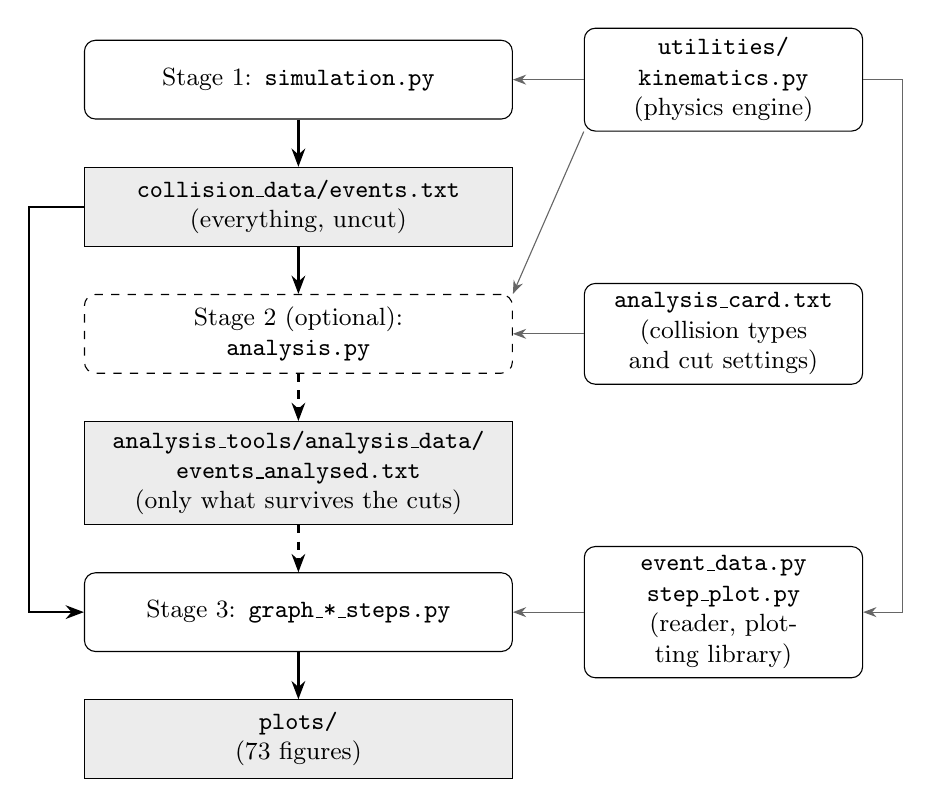
\begin{tikzpicture}[
    node distance=0.6cm and 0.9cm,
    proc/.style={rectangle, draw, rounded corners, text width=5.2cm, minimum height=1cm, align=center, font=\small},
    data/.style={rectangle, draw, fill=gray!15, text width=5.2cm, minimum height=1cm, align=center, font=\small},
    side/.style={rectangle, draw, rounded corners, text width=3.3cm, minimum height=1cm, align=center, font=\small},
    arr/.style={-{Stealth}, thick},
    dep/.style={-{Stealth}, thin, draw=black!60}
]
\node[proc] (sim) {Stage 1: \texttt{simulation.py}};
\node[data, below=of sim] (ev) {\texttt{collision\_data/events.txt}\\(everything, uncut)};
\node[proc, dashed, below=of ev] (ana) {Stage 2 (optional):\\\texttt{analysis.py}};
\node[data, below=of ana] (evan) {\texttt{analysis\_tools/\allowbreak analysis\_data/\allowbreak events\_analysed.txt}\\(only what survives the cuts)};
\node[proc, below=of evan] (plot) {Stage 3: \texttt{graph\_*\_steps.py}};
\node[data, below=of plot] (figs) {\texttt{plots/}\\(73 figures)};
\node[side, right=of sim] (kin) {\texttt{utilities/\allowbreak kinematics.py}\\(physics engine)};
\node[side, right=of ana] (card) {\texttt{analysis\_card.txt}\\(collision types and cut settings)};
\node[side, right=of plot] (edata) {\texttt{event\_data.py}\\\texttt{step\_plot.py}\\(reader, plotting library)};

\draw[dep] (kin) -- (sim);
\draw[dep] (kin.south west) -- (ana.north east);
\draw[dep] (kin.east) -- ++(0.5,0) |- (edata.east);
\draw[arr] (sim) -- (ev);
\draw[arr] (ev) -- (ana);
\draw[dep] (card) -- (ana);
\draw[arr, dashed] (ana) -- (evan);
\draw[arr, dashed] (evan) -- (plot);
\draw[arr] (ev.west) -- ++(-0.7,0) |- (plot.west);
\draw[dep] (edata) -- (plot);
\draw[arr] (plot) -- (figs);
\end{tikzpicture}
\caption{Data flow through the program. Grey boxes are files, white boxes are scripts, and the boxes on the right are supporting modules and settings. Thick arrows show the flow of event data, and thin arrows show the modules and settings on which each script depends. Besides generating the momenta, \texttt{kinematics.py} supplies the transverse momentum and pseudorapidity used by both \texttt{analysis.py} and \texttt{event\_data.py}. Dashed elements are optional: by default the plotting stage reads the uncut \texttt{events.txt}, and it reads the cut dataset only after the path \texttt{DATA\_FILE} at the top of each script is changed.}
\label{fig:chart_flow}
\end{figure}
\FloatBarrier

\section{Example of Numerical Results}
\label{sec:numerical_results}
The results in this section come from a dedicated run of 1{,}000{,}000 events, generated by \texttt{simulation.py} with the default settings and the default seed (2026), and analyzed by \texttt{analysis.py} with the default cuts. This dataset occupies about 500~MB, which is too large to distribute with the code; hence, the 100{,}000-event file \texttt{collision\_data/events.txt} is supplied with the program. \secref{ssec:dataset} describes the generated dataset, \secref{ssec:cut_effect} shows how many events survive the default cuts, and \secref{ssec:ee_example} presents distributions for one example process, $pp \to e^+e^-pp$, drawn from the events that pass all of the cuts.

\subsection{The Generated Dataset}
\label{ssec:dataset}
Table~\ref{tab:dataset} lists the number of events generated in each channel, before any cut is applied. The comparison with the sampling probabilities must be made at this stage, since the cuts accept the six channels with different efficiencies (\secref{ssec:cut_effect}) and would therefore change their relative fractions.

\begin{table}[H]
\centering
\begin{tabular}{l c c r c}
\hline
Process & ID & Probability & Events & Observed fraction \\
\hline
$pp$              & 1 & 0.25 & 250{,}479 & 0.2505 \\
$pp\gamma$        & 2 & 0.22 & 220{,}598 & 0.2206 \\
$ppn\overline{n}$ & 3 & 0.18 & 179{,}344 & 0.1793 \\
$ppe^+e^-$        & 4 & 0.15 & 149{,}871 & 0.1499 \\
$pp\mu^+\mu^-$    & 5 & 0.15 & 150{,}009 & 0.1500 \\
$pp\gamma\gamma$  & 6 & 0.05 & 49{,}699  & 0.0497 \\
\hline
All               &   & 1.00 & 1{,}000{,}000 & 1.0000 \\
\hline
\end{tabular}
\caption{Number of events generated in each channel of the 1{,}000{,}000-event dataset, before any cut, compared with the sampling probabilities.}
\label{tab:dataset}
\end{table}

Because the generator is random, the observed counts $N_i$ fluctuate around their expected values $N p_i$, where $N = 1{,}000{,}000$ and $p_i$ are the sampling probabilities of Table~\ref{tab:channels}. To test whether these fluctuations are of the expected size, we use Pearson's $\chi^2$ statistic for the chi-square goodness-of-fit test,
\begin{equation}
    \chi^2 = \sum_{i=1}^{6} \frac{\left(N_i - N p_i\right)^2}{N p_i},
\end{equation}
which has $6 - 1 = 5$ degrees of freedom, which means $\chi^2/dof=1.37$. Our dataset gives $\chi^2 = 6.86$. The corresponding $p$-value is $p = 0.23$: a generator sampling exactly these probabilities would produce a $\chi^2$ at least this large in $23\%$ of runs, purely by chance. This is well above the conventional threshold of $0.05$, so the observed fractions are consistent with the sampling probabilities.

\subsection{Effect of the Default Cuts}
\label{ssec:cut_effect}
Table~\ref{tab:acceptance} shows the fraction of events that survive the default cuts in each channel. Overall, $926{,}892$ of the $1{,}000{,}000$ events ($92.7\%$) are kept, and these form the cut dataset \texttt{events\_analysed.txt} from which the distributions of \secref{ssec:ee_example} are drawn. The $pp$ channel is affected least ($98.6\%$): both protons carry $6.8$~TeV, so the $p_T$ cut removes almost nothing ($99.99\%$ of events pass it), and the losses come from the pseudorapidity cut alone. The four-particle channels lose the most, about $11\%$, because an event is rejected if any one of its four particles fails a cut. These four channels have nearly identical acceptance, between $88.9\%$ and $89.0\%$, as expected: since every outgoing particle is massless, the kinematics do not depend on the particle species. The two cuts overlap, since both remove particles close to the beam axis, so the combined loss ($7.3\%$) is smaller than the sum of the separate losses ($3.8\% + 4.2\%$).

\begin{table}[H]
\centering
\begin{tabular}{l c r r r r}
\hline
Process & ID & Generated & $|\eta| < 2.5$ & $p_T \ge 0.1$~TeV & Both cuts \\
\hline
$pp$              & 1 & 250{,}479 & 98.61\% & 99.99\% & 98.61\% \\
$pp\gamma$        & 2 & 220{,}598 & 96.35\% & 98.23\% & 94.92\% \\
$ppn\overline{n}$ & 3 & 179{,}344 & 95.11\% & 92.79\% & 88.92\% \\
$ppe^+e^-$        & 4 & 149{,}871 & 95.07\% & 92.89\% & 89.02\% \\
$pp\mu^+\mu^-$    & 5 & 150{,}009 & 95.04\% & 92.82\% & 88.96\% \\
$pp\gamma\gamma$  & 6 & 49{,}699  & 94.98\% & 92.87\% & 88.88\% \\
\hline
All               &   & 1{,}000{,}000 & 96.24\% & 95.82\% & 92.69\% \\
\hline
\end{tabular}
\caption{Fraction of events kept by the default cuts, applied separately and together, for each channel of the 1{,}000{,}000-event dataset. An event is kept only if every one of its outgoing particles passes.}
\label{tab:acceptance}
\end{table}

\subsection{Example: the Process $pp \to e^+e^-pp$}
\label{ssec:ee_example}
As an example of the distributions the program produces, we show results for the four-particle process $pp \to e^+e^-pp$ (ID 4). Of the 149{,}871 events of this process generated, 133{,}408 ($89.0\%$) pass all of the default cuts, and only these events are used in the figures below; each figure was produced by the Stage~3 plotting scripts from the cut dataset. In this process the positron and the electron (particles 3 and 4) come from one composite system, of mass $m_{34}$, and the two final-state protons (particles 5 and 6) from the other, of mass $m_{56}$. Each figure shows all four outgoing particles, or both pairs, so that they can be compared directly, and its lower panel shows each curve divided by the first.

\subsubsection{Transverse Momentum of the Positron}
\label{sssec:result_pt}
Figure~\ref{fig:ee_pt} shows the transverse momentum of the four outgoing particles; the positron is the solid blue curve. Since every particle in these events has passed the cut $p_T \ge 0.1$~TeV, all four distributions begin at the dashed line. The positron distribution is a broad hump, roughly level between about $2.5$ and $4$~TeV, with a mean of $3.23$~TeV and a median of $3.19$~TeV. It extends up to about $6.8$~TeV, which is the largest transverse momentum a massless particle can have: at most half of the collision energy, $\sqrt{s}/2$, emitted perpendicular to the beam.

The electron follows the same distribution, and the ratio of the two stays close to 1 across the whole range: the two leptons are the decay products of the same composite system, decayed isotropically in its rest frame, so nothing distinguishes one from the other. The two protons, by contrast, are concentrated at low transverse momentum, peaking just above the cut and falling steadily, with a mean of $2.20$~TeV. This is the asymmetry of \secref{ssec:dataset}: the proton pair comes from the lighter composite on average, and so carries less energy.

\begin{figure}[H]
\centering
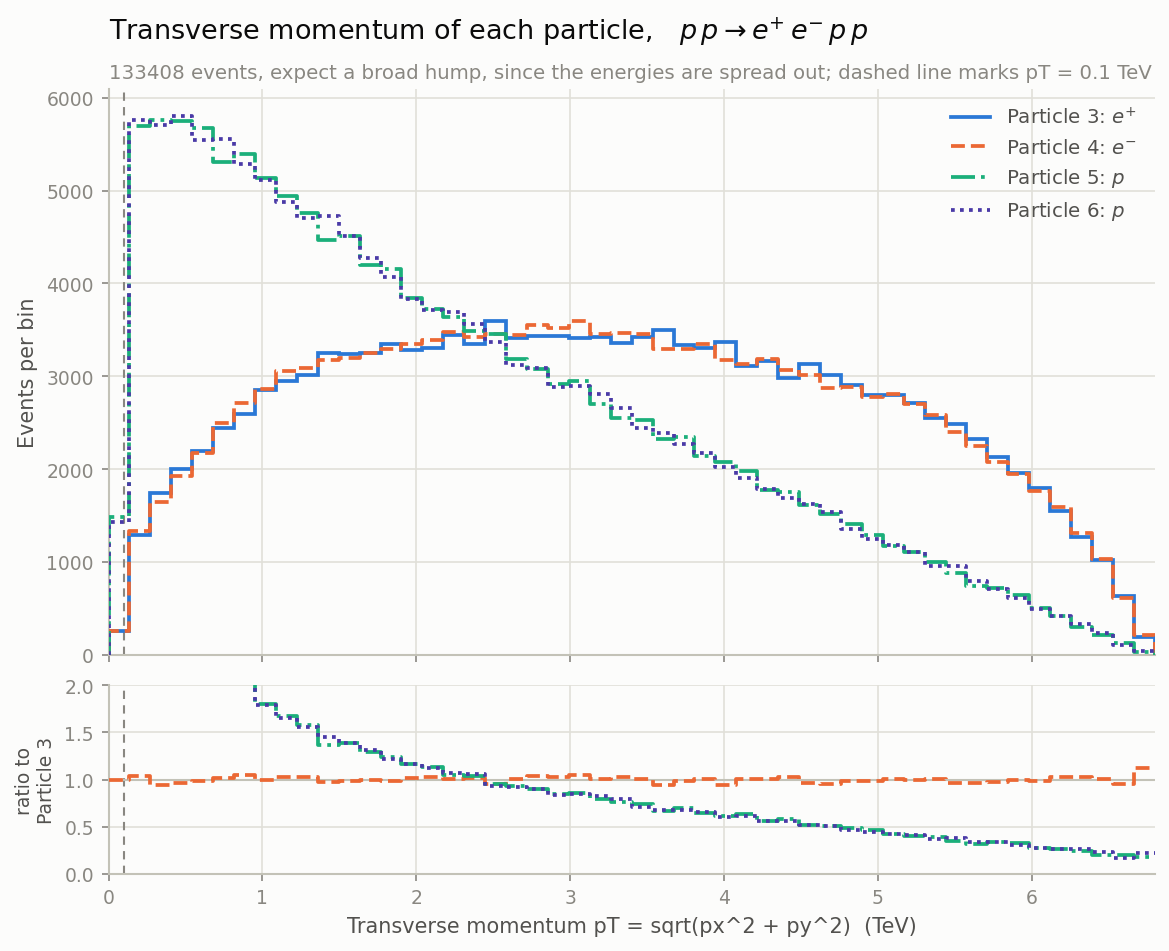
\includegraphics[width=0.9\textwidth]{figures/ee_transverse_momentum.png}
\caption{Transverse momentum of the four outgoing particles in $pp \to e^+e^-pp$, for the 133{,}408 events that pass all of the default cuts. The positron is the solid blue curve (particle 3) and the electron the dashed orange curve (particle 4); the two protons are the dash-dotted green and dotted purple curves. The dashed vertical line marks the cut $p_T = 0.1$~TeV, below which no particle survives. The lower panel shows each distribution divided by that of the positron; at low $p_T$ the proton ratios exceed 2 and lie above the top of the panel.}
\label{fig:ee_pt}
\end{figure}

\subsubsection{Pseudorapidity of the Electron}
\label{sssec:result_eta}
Figure~\ref{fig:ee_eta} shows the pseudorapidity of the four outgoing particles; the electron is the dashed orange curve. The pseudorapidity cut removes every particle beyond $|\eta| = 2.5$, so all four distributions stop sharply at the dashed lines. Within this range the electron distribution is symmetric about $\eta = 0$, with a mean of $+0.001$ and a standard deviation of $0.83$, and falls off steadily towards the edges of the acceptance. This is the shape expected for directions distributed isotropically: since $\cos\theta = \tanh\eta$, a uniform distribution of $\cos\theta$ becomes $\mathrm{d}N/\mathrm{d}\eta \propto 1/\cosh^2\eta$. For an isotropic distribution restricted to $|\eta| < 2.5$, a fraction $\tanh 1 / \tanh 2.5 = 77.2\%$ of particles would lie within $|\eta| < 1$; we observe $77.6\%$. The small excess arises because the $p_T$ cut also removes particles preferentially close to the beam axis, where $\sin\theta$, and hence $p_T = E\sin\theta$, is small.

All four particles share the same pseudorapidity distribution, and the ratio panel stays flat at 1 except in the sparsely populated bins at the edges of the acceptance. Although each particle's momentum is obtained through one or more Lorentz boosts, every direction in the generation is drawn isotropically, so the event as a whole has no preferred direction.

\begin{figure}[H]
\centering
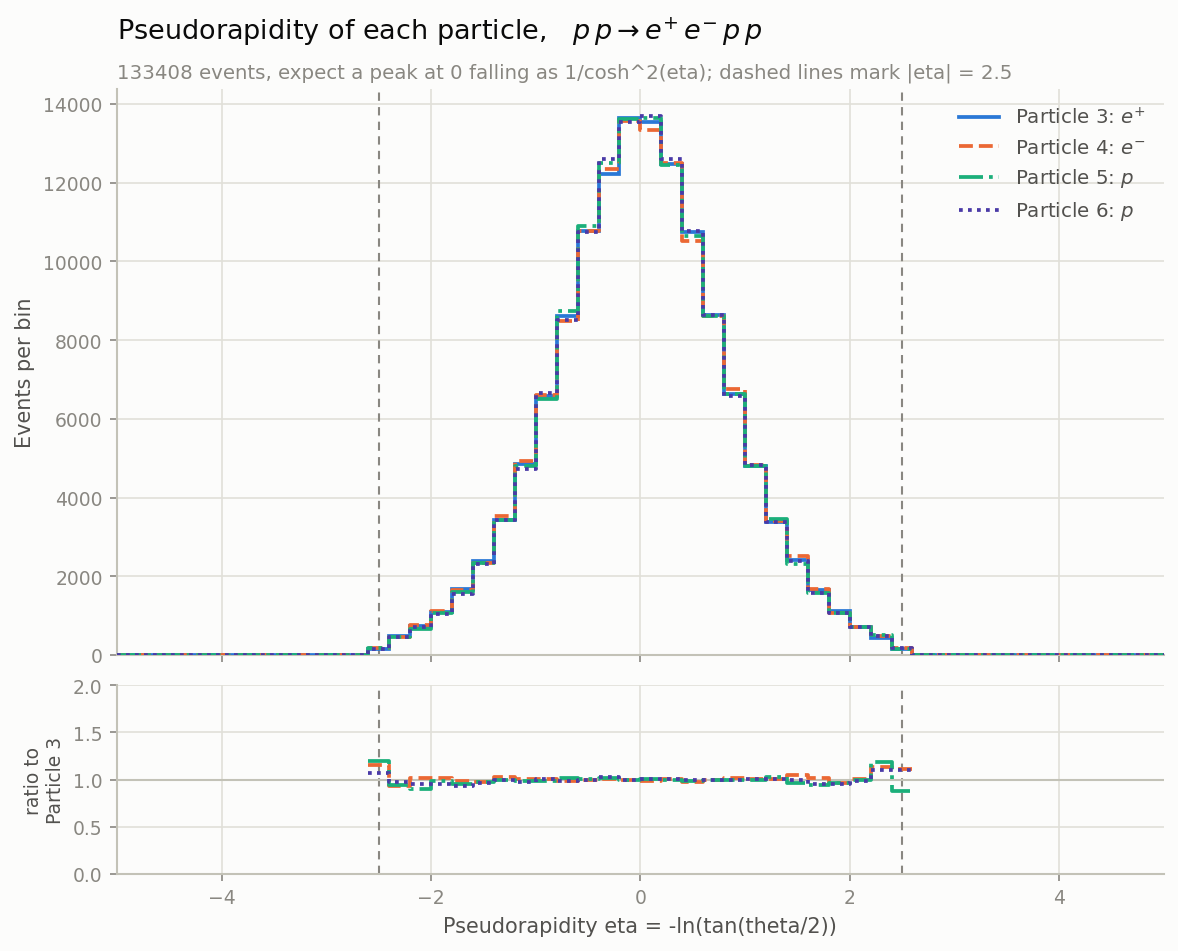
\includegraphics[width=0.9\textwidth]{figures/ee_pseudorapidity.png}
\caption{Pseudorapidity of the four outgoing particles in $pp \to e^+e^-pp$, for the 133{,}408 events that pass all of the default cuts. The electron is the dashed orange curve (particle 4). The dashed vertical lines mark the acceptance $|\eta| = 2.5$, beyond which no particle survives. The lower panel shows each distribution divided by that of the positron.}
\label{fig:ee_eta}
\end{figure}

\subsubsection{Invariant Masses of the $e^+e^-$ Pair and of the Final-State Proton Pair}
\label{sssec:result_mass}
Figure~\ref{fig:ee_mass} shows the invariant mass of the $e^+e^-$ pair (solid blue) and of the final-state proton pair (dashed orange), each reconstructed from the outgoing four-vectors as in \secref{sec:kinematics_framework}. Each pair came out of a single composite system, so its invariant mass reproduces the composite mass that the generator drew, $m_{34}$ for the leptons and $m_{56}$ for the protons, up to the few-GeV rounding of the output file.

As drawn by the generator, the $e^+e^-$ mass is distributed uniformly between $0$ and $13.6$~TeV, with an expected mean of $6.80$~TeV. After the cuts it remains flat up to about $12$~TeV, but falls away above that, and its mean drops to $6.51$~TeV; the fraction of pairs above $10$~TeV falls from the $26.5\%$ of a uniform distribution to $22.8\%$. This loss is caused by the cuts acting on the other two particles. When the $e^+e^-$ pair takes almost all of the collision energy, very little remains for the proton pair, whose mass $m_{56}$ is at most $\sqrt{s} - m_{34}$; its protons are then soft, fail the cut $p_T \ge 0.1$~TeV, and take the whole event with them.

The proton-pair mass falls steeply from zero, with a mean of $3.56$~TeV and a median of $2.77$~TeV; $22.2\%$ of proton pairs lie below $1$~TeV. Its shape follows from the sequential mass sampling of \secref{ssec:event_generation}: $m_{34}$ is drawn from the full range, whereas $m_{56}$ is drawn only from the range that remains. The ratio panel shows the proton-pair distribution falling below the lepton-pair one above about $5$~TeV.

Neither distribution shows a resonance peak, because the simulation contains no intermediate resonance particles. In a real $e^+e^-$ mass spectrum, for example, the $Z$ boson would appear as a narrow peak at $91$~GeV. The shapes in Figure~\ref{fig:ee_mass} therefore reflect the sampling assumptions of the generator and the effect of the cuts, rather than the dynamics of a real collision.

\begin{figure}[H]
\centering
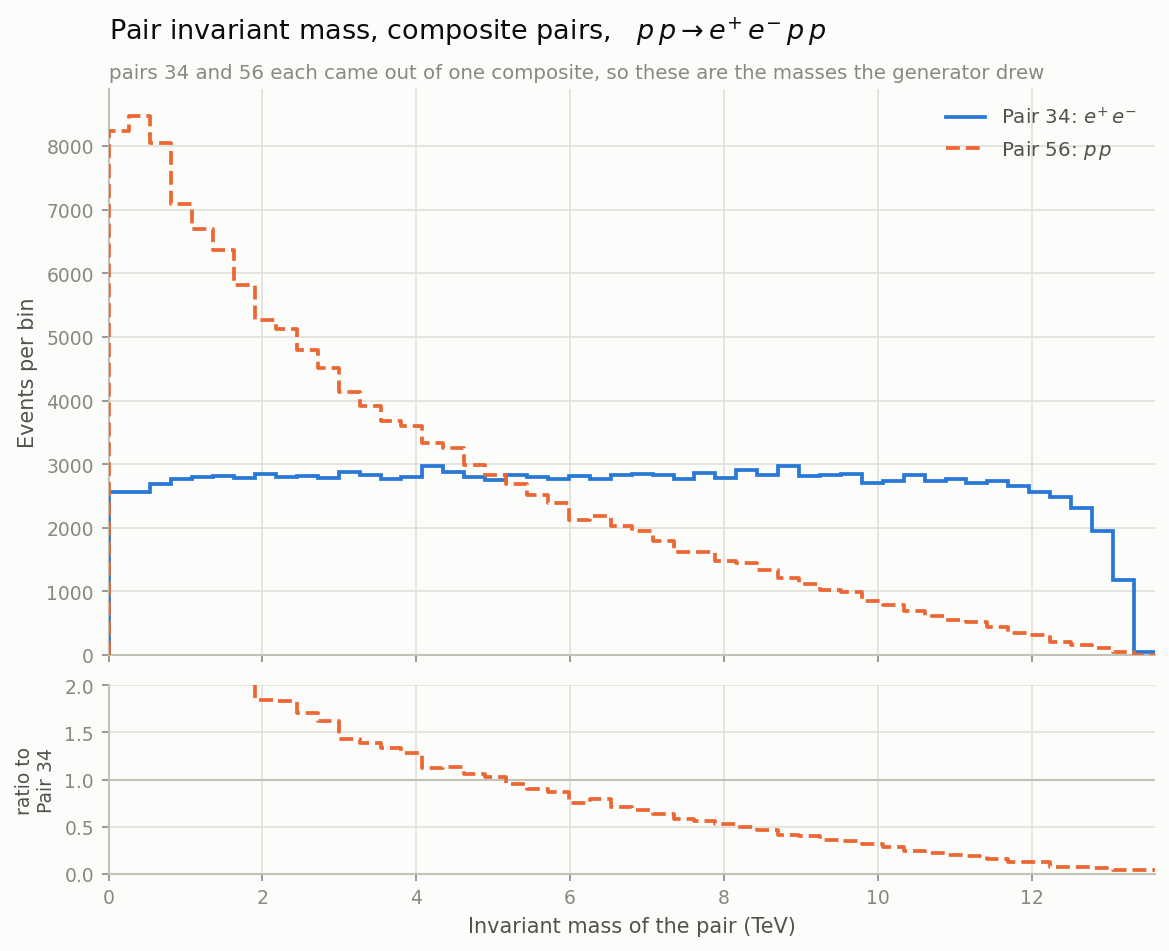
\includegraphics[width=0.9\textwidth]{figures/ee_invariant_mass.png}
\caption{Invariant mass of the $e^+e^-$ pair (pair 34, solid blue) and of the final-state proton pair (pair 56, dashed orange) in $pp \to e^+e^-pp$, for the 133{,}408 events that pass all of the default cuts. The lower panel shows the proton-pair distribution divided by the lepton-pair one; below about $1.9$~TeV the ratio exceeds 2 and lies above the top of the panel.}
\label{fig:ee_mass}
\end{figure}
\FloatBarrier

\section{Summary and Outlook}
\label{sec:conclusion}

\subsection{Conclusion}
We have presented a simplified Monte Carlo simulation of proton--proton collisions at the LHC, LASPOS, designed as an educational tool and released openly on GitHub. The program generates events for six final states containing two to four particles at any given collision energy. Multi-particle final states are reduced to a chain of exactly solvable two-body decays; composite systems are decayed in their own rest frames and boosted back to the laboratory frame with the general $4\times4$ Lorentz boost matrix (\secref{sec:kinematics_framework} and Appendices~\ref{app:2to2}--\ref{app:2to4}). As a result, every generated event conserves energy and momentum by construction, and the final-state menu is chosen so that electric charge, baryon number, and lepton number are conserved as well. The program is split into three independent stages --- event generation, detector cuts, and plotting --- so that a different set of cuts can be tested on the same events without regenerating them, and any distribution of the events, such as particle energies, angles, transverse momenta, and invariant masses, can be plotted (\secref{sec:user_guide} and \secref{sec:numerical_results}).

\par The simulation is deliberately simplified, and its distributions are illustrative rather than predictive. The relative frequencies of the final states are specified in advance rather than derived from a realistic theoretical model. Composite masses and emission directions are drawn from uniform or isotropic distributions instead of being derived from matrix elements; all outgoing particles, including the protons, are treated as massless; and no resonance is simulated, so the diphoton invariant-mass distribution contains no Higgs peak. These limitations indicate the directions in which the program can be extended.

\subsection{Outlook}
\par\textbf{Beyond uniform random numbers.} The first improvement is to replace the uniform draws by distributions that follow from the physics. In a real collision the probability of a configuration is set by the matrix element of the process and by the available phase space, so composite masses and emission angles could be drawn from the corresponding differential cross sections, and the chosen probabilities of the final states replaced by computed probabilities. Resonance-shaped distributions, such as a Breit--Wigner form, would allow a Higgs boson decaying to two photons to appear as a narrow peak near 125 GeV in the diphoton invariant mass, as in the discovery analyses \cite{atlas_higgs, cms_higgs}. It would also be natural to draw the two composite masses of the 2-to-4 case jointly rather than one after the other, which removes the bias that currently makes the second composite systematically lighter than the first.

\par\textbf{More final states.} The menu of six final states can be extended to include mesons, such as pions and kaons, the heavier lepton $\tau^\pm$, and neutrinos.

\par\textbf{Parton-level collisions.} A proton is a bundle of quarks and gluons (\secref{sec:theoretical_background}), so a proton--proton collision is in reality a collision between two partons, one from each proton. The present program ignores this substructure. A more realistic version would break each collision down into quark--quark, quark--gluon, and gluon--gluon collisions.

\newpage
\appendix
\section{Detailed Derivation: Two-Body Kinematics (2-to-2)}
\label{app:2to2}
This appendix gives the full derivation of the two-body kinematic relations summarized in \secref{sssec:2to2}, for the process $p_1 + p_2 \rightarrow B + C$ in the center-of-mass frame of $P_1$ and $P_2$ (the lab frame).

\subsection{Setup}
The incoming energy-momentum four-vectors are
\begin{equation}
    P_{1\mu} = (E, 0, 0, E), \qquad P_{2\mu} = (E, 0, 0, -E),
\end{equation}
so that the total energy is $2E$ and the total momentum vanishes,
\begin{equation}
    \vec{p}_1 + \vec{p}_2 = 0.
\end{equation}
By momentum conservation, the outgoing particles $B$ and $C$ must also satisfy
\begin{equation}
    \vec{p}_B + \vec{p}_C = \vec{p}_1 + \vec{p}_2 = 0 \quad \Rightarrow \quad \vec{p}_B = -\vec{p}_C,
\end{equation}
so the two outgoing momenta are equal in magnitude and opposite in direction:
\begin{equation}
    |\vec{p}_B| = |\vec{p}_C| \equiv |\vec{p}|.
\end{equation}

\subsection{Massless Case}
If both outgoing particles are massless, $P_B^2 = P_C^2 = 0$, so
\begin{equation}
    E_B^2 - |\vec{p}_B|^2 = 0 \quad \Rightarrow \quad E_B = |\vec{p}_B|,
\end{equation}
and similarly $E_C = |\vec{p}_C|$. Since $|\vec{p}_B| = |\vec{p}_C|$, it follows immediately that
\begin{equation}
    E_B = E_C.
\end{equation}
Energy conservation, $E_B + E_C = 2E$, then fixes
\begin{equation}
    E_B = E_C = E.
\end{equation}
The direction of $\vec{p}_B$ is not constrained by conservation laws alone; it is drawn isotropically (\secref{para:isotropic}), with $\theta_B \in [0,\pi]$ and $\varphi_B \in [0, 2\pi)$, and $C$ is emitted back-to-back, $\theta_C = \pi - \theta_B$, $\varphi_C = \varphi_B + \pi$, consistent with $\vec{p}_B = -\vec{p}_C$.

\subsection{Massive Case}
If $B$ and $C$ carry masses $m_B \neq m_C$, the on-shell (mass-shell) conditions are
\begin{equation}
    E_B^2 - |\vec{p}|^2 = m_B^2, \qquad E_C^2 - |\vec{p}|^2 = m_C^2,
\end{equation}
using $|\vec{p}_B| = |\vec{p}_C| = |\vec{p}|$. Subtracting the second equation from the first eliminates $|\vec{p}|^2$:
\begin{equation}
    E_B^2 - E_C^2 = m_B^2 - m_C^2.
\end{equation}
The left-hand side factors as a difference of squares:
\begin{equation}
    (E_B + E_C)(E_B - E_C) = m_B^2 - m_C^2.
\end{equation}
Using energy conservation, $E_B + E_C = 2E$, this becomes
\begin{equation}
    E_B - E_C = \frac{m_B^2 - m_C^2}{2E}.
\end{equation}
This is now a linear system in $E_B$ and $E_C$:
\begin{equation}
    E_B + E_C = 2E, \qquad E_B - E_C = \frac{m_B^2 - m_C^2}{2E}.
\end{equation}
Adding and subtracting these two equations and dividing by 2 gives
\begin{equation}
\begin{gathered}
    E_B = \frac{1}{2}\left[2E + \frac{m_B^2 - m_C^2}{2E}\right], \\
    E_C = \frac{1}{2}\left[2E - \frac{m_B^2 - m_C^2}{2E}\right].
\end{gathered}
\end{equation}
As a consistency check, setting $m_B = m_C$ recovers $E_B = E_C = E$, matching the massless result above (which is itself the special case $m_B = m_C = 0$).

Once $E_B$ (and hence $|\vec{p}|$ via $|\vec{p}| = \sqrt{E_B^2 - m_B^2}$) is known, the momentum components follow from a randomly drawn emission direction $(\theta, \varphi)$, with $\theta \in [0,\pi]$ and $\varphi \in [0, 2\pi)$:
\begin{equation}
    p_{Bx} = |\vec{p}|\sin\theta\cos\varphi, \qquad p_{By} = |\vec{p}|\sin\theta\sin\varphi, \qquad p_{Bz} = |\vec{p}|\cos\theta,
\end{equation}
with $C$ emitted back-to-back, $p_{Cx} = -p_{Bx}$, $p_{Cy} = -p_{By}$, $p_{Cz} = -p_{Bz}$.

\section{Detailed Derivation: Three-Body Final States (2-to-3)}
\label{app:2to3}
This appendix gives the full derivation of the three-body kinematic procedure summarized in \secref{para:2to3}, for the process $p_1 + p_2 \rightarrow 3 + 4 + 5$, in the lab frame.

\subsection{Reduction to an Effective Two-Body Process}
Energy and momentum conservation require
\begin{equation}
\begin{gathered}
    E_1 + E_2 = E_3 + E_4 + E_5 = 2E, \\
    \vec{p}_1 + \vec{p}_2 = \vec{p}_3 + \vec{p}_4 + \vec{p}_5 = 0.
\end{gathered}
\end{equation}
Rather than distributing the energy among three particles directly, particles 4 and 5 are grouped into a single composite system, labeled $(45)$, with four-momentum
\begin{equation}
    \vec{p}_{45} = \vec{p}_4 + \vec{p}_5, \qquad E_{45} = E_4 + E_5,
\end{equation}
and invariant mass $m_{45}$, drawn randomly in the range
\begin{equation}
    m_{45} \in [0, 2E].
\end{equation}
With this relabeling, the original three-body process is rewritten as an effective two-body process,
\begin{equation}
    p_1 + p_2 \rightarrow 3 + (45),
\end{equation}
where particle 3 is taken to be massless ($m_3 = 0$, e.g.\ a photon) and $(45)$ is treated as a single particle of mass $m_{45}$. This effective process satisfies momentum conservation by construction, since
\begin{equation}
    \vec{p}_3 + \vec{p}_{45} = \vec{p}_3 + \vec{p}_4 + \vec{p}_5 = \vec{p}_1 + \vec{p}_2 = 0.
\end{equation}

\subsection{Step 1: Energies of Particle 3 and the (45) System}
Applying the massive two-body result of Appendix \ref{app:2to2}, with $B = 3$ ($m_3 = 0$) and $C = (45)$ (mass $m_{45}$), gives
\begin{equation}
\begin{gathered}
    E_3 = \frac{1}{2}\left[2E + \frac{0 - m_{45}^2}{2E}\right] = \frac{1}{2}\left[2E - \frac{m_{45}^2}{2E}\right], \\
    E_{45} = \frac{1}{2}\left[2E + \frac{m_{45}^2}{2E}\right].
\end{gathered}
\end{equation}
A random emission direction $(\theta_3, \varphi_3)$, with $\theta_3 \in [0,\pi]$ and $\varphi_3 \in [0, 2\pi)$, is drawn for particle 3, with the $(45)$ system emitted back-to-back, $\theta_{45} = \pi - \theta_3$, $\varphi_{45} = \varphi_3 + \pi$, so that
\begin{equation}
\begin{gathered}
    p_{3x} = |\vec{p}_3|\sin\theta_3\cos\varphi_3, \qquad p_{3y} = |\vec{p}_3|\sin\theta_3\sin\varphi_3, \\ p_{3z} = |\vec{p}_3|\cos\theta_3, \qquad |\vec{p}_3| = E_3,
\end{gathered}
\end{equation}
using $E_3 = |\vec{p}_3|$ since particle 3 is massless. The $(45)$ system's four-momentum follows from $\vec{p}_{45} = -\vec{p}_3$, giving
\begin{equation}
    P_{45} = (E_{45},\, p_{45x},\, p_{45y},\, p_{45z}).
\end{equation}

\subsection{Step 2: Decay of the (45) System in Its Rest Frame}
The $(45)$ system is now decayed into particles 4 and 5. This is done most simply in the rest frame of $(45)$, where by definition its spatial momentum vanishes (spatial means $x$, $y$, and $z$ components):
\begin{equation}
    P'_{45} = (m_{45},\, 0,\, 0,\, 0).
\end{equation}
The energy of $(45)$ in its rest frame is $E'_{45}=m_{45}$, because the invariant mass is the same in every frame and is therefore unchanged by the Lorentz boost of Eq.~\ref{equa:matrixa}:
\begin{equation}
    P'^2_{45} = E'^2_{45} - |\vec{p}'_{45}|^2 = m_{45}^2, \qquad \vec{p}'_{45} = 0 \quad \Rightarrow \quad E'_{45} = m_{45}.
\end{equation}
In this frame, particles 4 and 5 are emitted back-to-back, exactly as in the massless two-body case of Appendix~\ref{app:2to2} (with $m_{45}$ playing the role of the total energy budget $2E$ in that derivation). This gives
\begin{equation}
    E'_4 = E'_5 = \frac{m_{45}}{2},
\end{equation}
with an isotropic random emission direction $(\theta'_4, \varphi'_4)$ (\secref{para:isotropic}), with $\theta'_4 \in [0,\pi]$ and $\varphi'_4 \in [0, 2\pi)$, so that
\begin{equation}
    p'_{4x} = \frac{m_{45}}{2}\sin\theta'_4\cos\varphi'_4, \quad p'_{4y} = \frac{m_{45}}{2}\sin\theta'_4\sin\varphi'_4, \quad p'_{4z} = \frac{m_{45}}{2}\cos\theta'_4,
\end{equation}
and particle 5 emitted oppositely, $\vec{p}'_5 = -\vec{p}'_4$.

\subsection{Step 3: Boosting Back to the Lab Frame}
The primed quantities $P'_4 = (E'_4, p'_{4x}, p'_{4y}, p'_{4z})$ are defined in the rest frame of $(45)$ and must be boosted back to the lab frame $R_{12}$ (the center-of-mass frame of the incoming particles). Using the boost matrix $[A]$ of \secref{sssec:lorentz}, constructed from the lab-frame four-momentum $P_{45}$ obtained in Step 1,
\begin{equation}
    P_4 = [A]\, P'_4, \label{equa:matrixa}
\end{equation}
where $[A]$ is built from $\beta_x = p_{45x}/E_{45}$, $\beta_y = p_{45y}/E_{45}$, $\beta_z = p_{45z}/E_{45}$, following \secref{sssec:lorentz}. Once $P_4$ is known, $P_5$ follows directly from momentum conservation in the lab frame,
\begin{equation}
    P_5 = P_{45} - P_4,
\end{equation}
without requiring a second, independent boost of $P'_5$ (though boosting $P'_5$ directly gives an equivalent result and serves as a useful numerical check).

\subsection{Summary of the Procedure}
\begin{enumerate}
    \item Draw $m_{45} \in [0, 2E]$ and $(\theta_3, \varphi_3) \in [0,\pi]\times[0,2\pi)$; compute $E_3$, $E_{45}$, and $P_{45}$.
    \item Draw $(\theta'_4, \varphi'_4) \in [0,\pi]\times[0,2\pi)$; compute $E'_4 = E'_5 = m_{45}/2$ and $P'_4$ in the $(45)$-rest frame.
    \item Boost $P'_4$ to the lab frame using $[A]$ built from $P_{45}$, obtaining $P_4$; recover $P_5 = P_{45} - P_4$.
\end{enumerate}

\section{Detailed Derivation: Four-Body Final States (2-to-4)}
\label{app:2to4}
This appendix gives the full derivation of the four-body kinematic procedure summarized in \secref{para:2to4}, for the process $p_1 + p_2 \rightarrow 3 + 4 + 5 + 6$, in the lab frame.

\subsection{Reduction to Two Composite Pairs}
Energy and momentum conservation require
\begin{equation}
\begin{gathered}
    E_1 + E_2 = E_3 + E_4 + E_5 + E_6 = 2E, \\
    \vec{p}_1 + \vec{p}_2 = \vec{p}_3 + \vec{p}_4 + \vec{p}_5 + \vec{p}_6 = 0.
\end{gathered}
\end{equation}
The four-body final state is grouped into two composite systems, $(34)$ and $(56)$, with
\begin{equation}
    P_{34} = (E_{34},\, p_{34x},\, p_{34y},\, p_{34z}), \qquad P_{56} = (E_{56},\, p_{56x},\, p_{56y},\, p_{56z}),
\end{equation}
and invariant masses $m_{34}$, $m_{56}$ drawn randomly subject to the constraint that the total energy budget is not exceeded,
\begin{equation}
    m_{34} \in [0, 2E], \qquad m_{56} \in [0,\, 2E - m_{34}],
\end{equation}
which guarantees $2E \geq m_{34} + m_{56}$, so that the effective two-body process below has a physically valid (non-negative) momentum solution. With this relabeling, the original four-body process becomes an effective two-body process,
\begin{equation}
    p_1 + p_2 \rightarrow (34) + (56),
\end{equation}
which satisfies momentum conservation by construction, since $\vec{p}_{34} + \vec{p}_{56} = \vec{p}_1 + \vec{p}_2 = 0$.

\subsection{Step 1: Energies of the (34) and (56) Systems}
Applying the massive two-body result of Appendix \ref{app:2to2}, with $B = (34)$ (mass $m_{34}$) and $C = (56)$ (mass $m_{56}$), gives
\begin{equation}
    E_{34} = \frac{1}{2}\left[2E + \frac{m_{34}^2 - m_{56}^2}{2E}\right], \qquad E_{56} = 2E - E_{34}.
\end{equation}
A random splitting direction $(\theta_{34}, \varphi_{34})$, with $\theta_{34} \in [0,\pi]$ and $\varphi_{34} \in [0, 2\pi)$, is drawn, with $(56)$ emitted back-to-back, $\theta_{56} = \pi - \theta_{34}$, $\varphi_{56} = \varphi_{34} + \pi$, giving the four-momenta
\begin{equation}
    P_{34} = (E_{34},\, p_{34x},\, p_{34y},\, p_{34z}), \qquad P_{56} = (E_{56},\, p_{56x},\, p_{56y},\, p_{56z}),
\end{equation}
using $|\vec{p}_{34}| = \sqrt{E_{34}^2 - m_{34}^2}$ and the drawn direction $(\theta_{34}, \varphi_{34})$, with $P_{56}$ fixed by $\vec{p}_{56} = -\vec{p}_{34}$.

\subsection{Step 2: Independent Decay of Each Composite}
Each composite is decayed independently, in its own rest frame, exactly as in Appendix~\ref{app:2to3}, Step 2. In the rest frame of $(34)$,
\begin{equation}
    P'_{34} = (m_{34},\, 0,\, 0,\, 0), \qquad E'_3 = E'_4 = \frac{m_{34}}{2},
\end{equation}
with a random direction $(\theta'_3, \varphi'_3)$, with $\theta'_3 \in [0,\pi]$ and $\varphi'_3 \in [0, 2\pi)$, fixing $\vec{p}'_3$, and $\vec{p}'_4 = -\vec{p}'_3$. Independently, in the rest frame of $(56)$,
\begin{equation}
    P'_{56} = (m_{56},\, 0,\, 0,\, 0), \qquad E'_5 = E'_6 = \frac{m_{56}}{2},
\end{equation}
with its own independently drawn random direction $(\theta'_5, \varphi'_5)$, with $\theta'_5 \in [0,\pi]$ and $\varphi'_5 \in [0, 2\pi)$, fixing $\vec{p}'_5$, and $\vec{p}'_6 = -\vec{p}'_5$. The two decays use independent random directions since $(34)$ and $(56)$ decay in unrelated rest frames.

\subsection{Step 3: Boosting Each Pair Back to the Lab Frame}
Each primed four-momentum is boosted back to the lab frame $R_{12}$ using a boost matrix constructed from its own parent composite's lab-frame four-momentum. For particle 3,
\begin{equation}
    P_3 = [A_{34}]\, P'_3,
\end{equation}
where $[A_{34}]$ is built from $\beta_x = p_{34x}/E_{34}$, $\beta_y = p_{34y}/E_{34}$, $\beta_z = p_{34z}/E_{34}$, following \secref{sssec:lorentz}. Particle 4 then follows from momentum conservation, $P_4 = P_{34} - P_3$. Similarly, for particle 5,
\begin{equation}
    P_5 = [A_{56}]\, P'_5,
\end{equation}
with $[A_{56}]$ built from $\beta_x = p_{56x}/E_{56}$, $\beta_y = p_{56y}/E_{56}$, $\beta_z = p_{56z}/E_{56}$, and particle 6 follows from $P_6 = P_{56} - P_5$.

\subsection{Summary of the Procedure}
\begin{enumerate}
    \item Draw $m_{34} \in [0, 2E]$, $m_{56} \in [0,\, 2E-m_{34}]$, and $(\theta_{34}, \varphi_{34}) \in [0,\pi]\times[0,2\pi)$; compute $E_{34}$, $E_{56}$, $P_{34}$, $P_{56}$.
    \item Draw $(\theta'_3, \varphi'_3)$ and $(\theta'_5, \varphi'_5)$ independently, each in $[0,\pi]\times[0,2\pi)$; compute $E'_3=E'_4=m_{34}/2$ and $E'_5=E'_6=m_{56}/2$ in each composite's rest frame.
    \item Boost $P'_3$ using $[A_{34}]$ and $P'_5$ using $[A_{56}]$; recover $P_4 = P_{34}-P_3$ and $P_6 = P_{56}-P_5$.
\end{enumerate}

\newpage
\bibliographystyle{unsrtnat}
\bibliography{references}

\end{document}